\documentclass[../main.tex]{subfiles}
\begin{document}
\chapter{Validazione del framework}
In questo capitolo verrà proposta una validazione di un deployment di test del framework Moon Cloud, mediante la valutazione della sicurezza tramite l'esecuzione del driver sviluppato a tutti i livelli dello stack cloud (infrastruttura, piattaforma, software). 

\section{Deployment di Moon Cloud}

Il deployment dell'ambiente di test è stato effettuato su un'architettura multi-layer così composta:
\begin{itemize}
    \item A livello di infrastruttura, un nodo fisico, Dell PowerEdge T430 equipaggiato con processore Intel(R) Xeon(R) CPU E5-2630 v4 (10 core fisici e 40 thread logici), 48GB di RAM e 5 dischi da 1TB ciascuno in configurazione RAID 1. Su questa macchina è stato installato il sistema operativo CentOS 7.2, e il software Open Stack Newton.
        Successivamente sono state create 3 macchine virtuali con sistema operativo CentOS 7.2, in un flavor con 4GB di RAM e 10GB di disco.
    \item A livello di piattaforma, un cluster Docker Swarm di 2 nodi per i componenti core di Moon Cloud. La terza macchina virtuale è stata utilizzata come nodo di esecuzione per un cluster di dimensione unaria.
    \item A livello software, i componenti di Moon Cloud: 7 servizi core, gestiti tramite container Docker sul cluster swarm e 3 microservizi per la gestione del nodo di esecuzione.
        \textbf{Componenti Core}
        \begin{itemize}
            \item API
            \item Database
            \item Repository
            \item Database \textit{time-series} per i risultati
            \item Evaluation Manager
            \item RabbitMQ per la comunicazione tra API e Container
            \item Traefik (reverse proxy) per l'esposizione delle API
        \end{itemize}
        \textbf{Componenti execution node e execution cluster}
        \begin{itemize}
            \item Execution Manager
            \item Monitor Execution Manager
            \item Traefik (reverse proxy) per l'esposizione di alcune tipologie di test
        \end{itemize}
\end{itemize}


\section{Sicurezza del deployment}
L'analisi della sicurezza è stata effettuata a livello di infrastruttura, analizzando le configurazioni sul sistema operativo del server fisico e le caratteristiche del setup OpenStack; a livello di piattaforma, analizzando le configurazioni del template utilizzato per le macchine virtuali Docker e i container Moon Cloud; a livello applicativo, analizzando la sicurezza nei meccanismi di integrazione dei vari componenti.
\subsection{Infrastruttura}
\subsubsection{Analisi OpenSCAP del server fisico}
\begin{comment}
test finished
started at 1496183480
ended at 1496184352
lasted -872 seconds
report available at
https://moonclouddashboard.blob.core.windows.net/pdfcontainer/f4a1943cff

\end{comment}
Il test è stato eseguito utilizzando il driver realizzato, specificando in input il documento XCCDF "ssg-centos7" unitamente al profilo "\textit{nist-800-171-cui}".
La valutazione delle OVAL mediante il driver realizzato è durata 872 secondi.
I risultati riportati segnalano:
\begin{itemize}
    \item 119 valutazioni effettuate con successo
    \item 72 valutazioni fallite
\end{itemize}
\begin{figure}[H]
    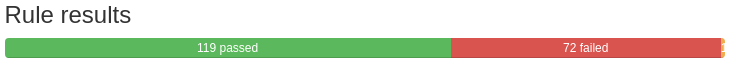
\includegraphics[width=10cm]{immagini/test_oscap_1.png}
\end{figure}

In particolare, delle 72 valutazioni fallite, 11 sono di severity bassa, 50 di severity media e 11 di severity elevata; lo score della copertura XCCDF ottenuto è 71.17\%.

\begin{figure}[H]
    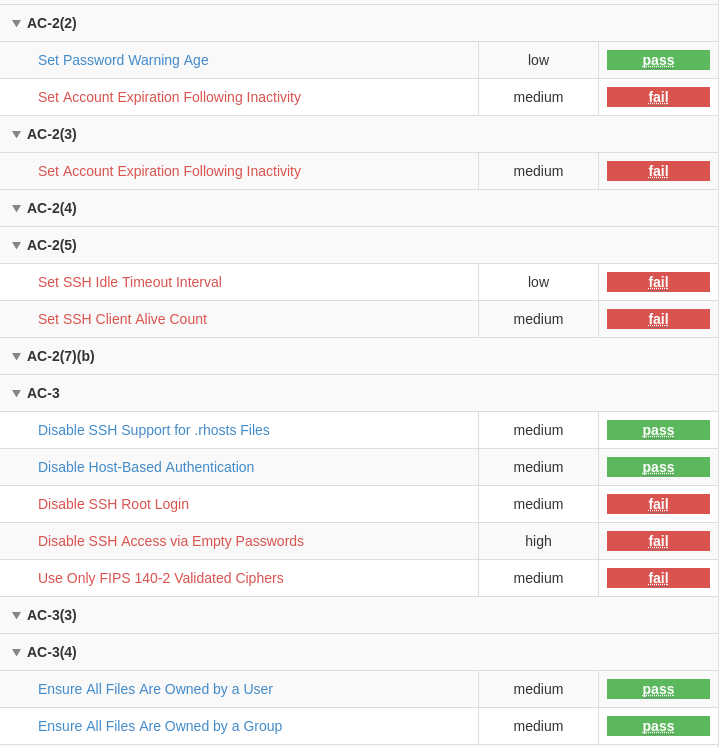
\includegraphics[width=10cm]{immagini/test_oscap_1_1.png}
    \label{Estratto del report}
\end{figure}

Il report completo è disponibile all'indirizzo:\\
\textit{https://moonclouddashboard.blob.core.windows.net/pdfcontainer/f4a1943cff}
\\
o, in alternativa, nel repository GIT\\
\textit{https://github.com/patriziotufarolo/tesi\_magistrale/}.

\subsubsection{Analisi di OpenStack}
I documenti XCCDF forniti da OpenSCAP non sono risultati efficienti per l'assessment dei controlli di sicurezza per Open Stack, in quanto le definizioni \textit{OVAL} non sono state redatte
Questa sezione, pertanto, fa riferimento al paper "A Security Benchmark for OpenStack". Ogni raccomandazione citata nell'articolo è mappata sui requisiti FedRAMP corrispondenti, ove possibile.

\begin{tabulary}{|c|c|c|}
    \textbf{[R1] Patch Levels.} & \textbf{Passato} &
    \textbf{[R2] Create and Enforce Account and Password Management Policies.} &
    \textbf{Fallito} \\ \hline
    \textbf{[R3] Use a Central Directory for Authentication and Authorization.} &
    \textbf{Fallito} \\ \hline 
    \textbf{[R4] Configure Firewalls to Restrict Access.} &
    \textbf{Fallito} &
    \textbf{[R5] Use TLS/SSL where Possible.} &
    \textbf{Fallito} &
    \textbf{[R6] Do Not Use Default Self-Signed Certificates.} &
    \textbf{Non applicabile} &
    \textbf{[R7] Configure Centralized Remote Logging.} &
    \textbf{Fallito} &
    \textbf{[R8] Maintain Time Synchronization Services.} &
    \textbf{Passato} &
    \textbf{[R9] Review and Minimize Hypervisor Attack Surface.} &
    \textbf{Non eseguito} &
    \textbf{[R10] Review and Minimize Virtual Machine Manager Attack Surface.} &
    \textbf{Non eseguito} &
\textbf{[R11] Use Templates to Deploy Virtual Machines.}
\textbf{Passato}
\textbf{[R12] Disconnect unauthorized devices from Virtual Machines.} 
\textbf{Non applicabile}
\textbf{[R13] Disable MAC Address Changes and Promiscuous Mode on Guests.} Hypervisor or Network virtualizators should deny MAC address changes on the Vnic (\emph{Virtual})
\textbf{Passato}
\textbf{[R14] Ensure Network Isolation through VLANs.} 
\textbf{Passato}
\textbf{[R15] Port Groups Should not be Configured to Reserved VLANs.}
\textbf{Passato}
\textbf{[R16] Secure Access to Cloud Application Programming Interfaces.} 
\textbf{Fallito}
\textbf{[R17] Encrypt Data at Rest.} 
\textbf{Fallito}
\textbf{[R18] Establish Appropriate Resource Isolation.} 
\textbf{Passato}
\textbf{[R19] Evaluate Denial of Service Scenarios and Mitigations.} 
\textbf{Fallito}
\textbf{[R20] Do Not Use or Set Guest Customization Passwords.}
\textbf{Passato}
\textbf{[R21] Evaluate and Minimize Cloud Architecture Dependencies.}
\textbf{Non eseguito}
\textbf{[R22] Audit Sensible and Configuration Files.} 
\textbf{Fallito}
\textbf{[R23] Storage Reliability.} 
\textbf{Fallito}
\textbf{[R24] Data Remanence Avoidance.}
\textbf{Fallito}

\subsection{Piattaforma}
\subsubsection{Analisi OpenSCAP sul template delle macchine virtuali}
test finished
started at 1496218136
ended at 1496218350
lasted -214 seconds

report available at
https://moonclouddashboard.blob.core.windows.net/pdfcontainer/b73210ae24
--

\subsubsection{Analisi dei container Moon Cloud}

\subsection{Applicazione}
\subsubsection{Analisi dei componenti software}

L'analisi effettuata sulla piattaforma Moon Cloud si è limitata allo studio della sicurezza nei canali di comunicazione e nei meccanismi di interazione tra i vari componenti.




\end{document}
